\section{Strumenti per la coordinazione}
\subsection{Gestione condivisione file}
Per gestire efficientemente la condivisione dei file intra-gruppo a supporto dello strumento di \textbf{Git} è stato scelto l'utilizzo di: Google Drive, un servizio \textit{web} di \textit{storage} e sincronizzazione \textit{online} che dovrebbe facilitare la condivisione e fornire una base d'appoggio secondaria ed informale per alcuni file che non necessitano versionamento.
L'utilizzo di \textit{Google Drive} e' limitato ai documenti che:
\begin{itemize}
\item Non necessitano di versionamento;
\item Necessitano di essere acceduti velocemente tramite \textit{web};
\end{itemize}

\subsection{Repository}
Di pressoché fondamentale importanza è stata la definizione di un ambiente ordinato in cui organizzare e mantenere tutti i \textit{file} che attraversano il ciclo di vita, per questa ragione è stato scelto di avvalersi di un \textit{repository}. 

\subsubsection{GitHub}
Come sistema di controllo di versione è stato adottato il software \textit{GitHub\ped{G}}, i pregi di questo strumento vengono qui di seguito riportati:
\begin{itemize}
\item Molto reattivo;
\item Design semplice; 
\item \textit{Software} gratuito.
\end{itemize}

\subsubsection{Struttura repository}
L'indirizzo di \textbf{root\ped{G}} del \textit{repository} contenente tutta la documentazione è:
\begin{center}
\href{https://github.com/Dquaglio/Sirius}{https://github.com/Dquaglio/Sirius}
\end{center}

Ogni documento presente sarà contenuto in una sotto cartella del \textit{master branch\ped{G}} nominata come il nome del documento stesso.
All'interno della cartella potranno essere contenuti solamente \textit{file.tex}, per la visualizzazione del relativo \textit{pdf\ped{G}} sarà necessario scaricarli e compilarli, assicurandosi di avere l'ultima versione del modello disponibile.
\begin{center}
\textbf{modello.git}: \href{https://github.com/Dquaglio/Sirius/tree/master/modello.git}{https://github.com/Dquaglio/Sirius/tree/master/modello.git}
\end{center}

conterrà il \textit{template} \LaTeX, le \textit{macro} e gli script aggiornati all'ultima versione disponibile.
\\
\\
Il \textit{master branch} è stato quindi suddiviso seguendo questa struttura:
\begin{figure}
\centering
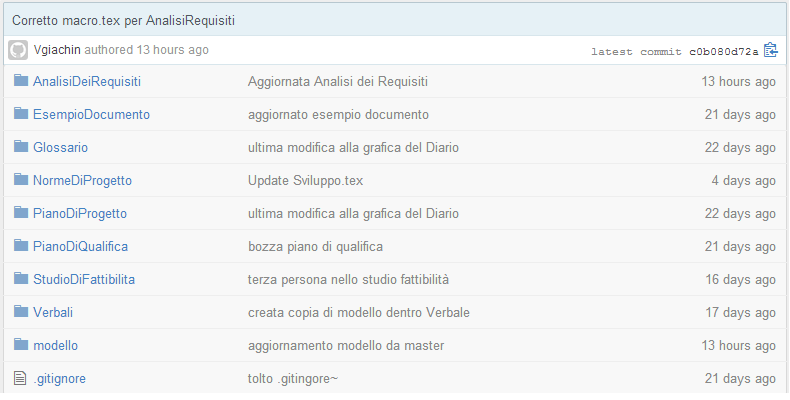
\includegraphics[width= %
\linewidth]{immaginiNDP/repository}
\caption[]{Struttura master branch.}
\label{fig:repository}
\end{figure}
A scopo puramente dimostrativo è stato creato l'esempio di un documento formale del gruppo \gruppo, contenuto nella cartella: "EsempioDocumento", questa scelta è stata fatta per illustrare la struttura generale che deve preservare qualsiasi documento (sezione 5.4, Struttura documentazione).
Per sfruttare il parallelismo nello sviluppo di uno stesso documento sono stati creati appositamente dei  \textit{branch} denominati con il nome dei membri del gruppo, i documenti  \textit{baseline\ped{G}} invece saranno contenuti solamente nel \textit{master branch}. Il \textit{merge\ped{G}} con il ramo \textit{master} avviene quindi solamente dopo la terminazione del processo di verifica di un documento.
